\section{Free selective functors}\label{sec-free}

Free construction with examples

The methodology of building effectful computations with free constructions such
as free~\cite{free-monads} and freer~\cite{freer-monads} monads and free
applicatives~\cite{free-applicatives} is a widespread in the functional programming community.
It allows to focus on the internal aspects of the effect under consideration and receive the
desired \hs{Applicative} of \hs{Monadic} structure of the computation~\emph{for free},
i.e. without the need to construct instances or prove laws.

In the ``free structures'' methodology, the essence of an effect is a datatype which encodes
the ``commands'' which the effect provides, acting as a deep embedding of the effect's
interface. This datatype must only have enough structure to be a~\hs{Functor}. The purpose of
the free constructions is then to build on top of this functor a richer structure,
which would have the instances of \hs{Applicative}/\hs{Selective}/\hs{Monad}.

\subsection{Free construction}\label{sec-free-construction}

...

\subsection{Ping-pong, freely}\label{sec-free-ping-pong}

To illustrate the usage of the free selective constructor on a simple example, we implement the
Teletype DSL~\cite{swierstra2008data} comprising two commands: reading a string of characters
form the input stream and writing a string to the output stream. The \hs{Teletype} datatype
has two constructors, representing the commands of the Teletype interface:

\begin{minted}[xleftmargin=10pt]{haskell}
data Teletype a = GetLine (String -> a)
                | PutStrLn String a
    deriving Functor
\end{minted}

We embed these commands into the free selective construction with the following two combinators,
mimicking Haskell Prelude's \hs{IO} API:

\begin{minted}[xleftmargin=10pt]{haskell}
getLine :: Select Teletype String
getLine = liftSelect (GetLine id)

putStrLn:: String -> Select Teletype ()
putStrLn s = liftSelect (PutStrLn s ())
\end{minted}

We now can reimplement the \hs{pingPongS} example from the section \ref{sec-intro}
in terms of the free selective construction simply by adjusting the type signature:

\begin{minted}[xleftmargin=10pt]{haskell}
pingPongS :: Select Teletype ()
pingPongS = whenS (fmap (=="ping") getLine) (putStrLn "pong")
\end{minted}

Once we have embedded the \hs{pingPongS} program into the \hs{Select} datatype,
we got access to the machinery for static analysis of effects:

\begin{minted}[xleftmargin=10pt]{haskell}
@\ghci@ getEffects pingPong
[GetLine,PutStrLn pong]
\end{minted}

The \hs{getEffects} function of type \hs{Functor f => Select f a -> [f ()]}
returns a list of all effects of a free selective computation. In the specific case of
the \hs{Teletype} functor, we get a list of all commands that a computation has called.
Internally, the \hs{getEffects} function interprets a free selective computation
in the \hs{Over} functor (see section~\ref{sec-instances}) to construct an over-approximated
list of effects.

We can interpret Teletype programs in any other \hs{Selective} by means of the
\hs{runSelect} function. We must providing a \emph{natural transformation}
\hs{forall a. f a -> g a}, which assigns an interpretation to the commands of
\hs{f} (in our example, \hs{f}~\hs{=}~\hs{Teletype}) in terms of \hs{g}.
A natural example of such a transformation would be an interpretation in the \hs{IO} monad,
which allows to run our \hs{pingPongS} program and get the same behaviour that the
one in \ref{sec-intro} had.

\begin{minted}[xleftmargin=10pt]{haskell}
inIO :: Teletype a -> IO a
inIO (GetLine t)    = t <$> Prelude.getLine
inIO (PutStrLn s x) = Prelude.putStrLn s *> pure x
\end{minted}

\subsection{Build systems, freely}\label{sec-free-build}

...

\subsection{Analysis and simulation of processor instructions}\label{sec-free-isa}

To apply free selective functors to a larger example, we demonstrate
how they can be used for describing the semantics of a hypothetical
instruction set architecture. The features of the free selective construction will
allow for static data-flow analysis of the instruction semantics, and the possibility
to interpret free selective expressions in any monad will enable us to build a
sequential simulator for programs.

\subsubsection{Embedding}

We will represent the semantics of instructions in terms of the following datatype:

\begin{minted}[xleftmargin=10pt]{haskell}
type ISA a = Select RW a
\end{minted}

Here, \hs{Select} is the free selective functor defined earlier in this section.
We apply the \hs{Select} type constructor to the \hs{RW} datatype, which is the
functor we build our free construction on:

\begin{minted}[xleftmargin=10pt]{haskell}
data RW a = Read  Key             (Value -> a)
          | Write Key (ISA Value) (Value -> a)
    deriving Functor
\end{minted}

The \hs{RW} (pronounced read-write) functor encodes the effect of mutable key-value store
comprising two commands.
First, we need to have an ability to \emph{read} a value associated with a key from the store
and second, given a computation which produces a value, \emph{write} its result into the store.
This exact structure of the definition is required for accommodating a pattern that
occurs frequently in instruction semantics: often we read a value from a register or a memory
cell, do something with the value and then write it somewhere else.
If we had the type of \hs{Write} to be \hs{k -> v -> (v -> a)}, i.e. required
the second argument to be a pure value,
we would not be able to grasp the desired pattern without resorting to the monadic interface.
Additionally, we want the \hs{Write}
operation to not just write the value and return \hs{()}, but to give the just written value
back, so it may be used in the rest of the computations; such a generosity of the \hs{Write}
command not consuming its arguments will be useful to avoid creating more data dependencies
than necessary.

We introduce two convenience combinators, which \emph{lift} the data constructors
of the \hs{RW} datatype into the free selective, thus making them directly usable in
the definitions of instruction semantics:

\begin{minted}[xleftmargin=10pt]{haskell}
read :: Key -> ISA Value
read k = liftSelect (Read k id)

write :: Key -> ISA Value -> ISA Value
write k p = p *> liftSelect (Write k p id)
\end{minted}

Whereas the \hs{read} combinator is exactly the lifted \hs{Read} data constructor,
the \hs{write}'s implementation deserves explanation, since it deviates from the trivial
lifting of the \hs{Write} data constructor and \emph{evaluates its second argument},
thus executing its associated effects.

\subsubsection{\textbf{Example 1. Addition}}

To get acquainted with the vocabulary, we start with a simple semantics for
the addition instruction, which will read the summands from a register and a memory cell,
add them, write the result back into the register and also update the state of the \hs{Zero}
and \hs{Overflow} flags to indicate if the sum was zero and if integer overflow occurred:

\begin{minted}[xleftmargin=10pt]{haskell}
add :: Register -> Address -> ISA Value
add reg addr = let arg1     = read (Reg reg)
                   arg2     = read (Mem addr)
                   result   = (+)  <$> arg1   <*> arg2
                   isZero   = (==) <$> pure 0 <*> write (Reg reg) result
                   overflow = willOverflowPure <$> arg1 <*> arg2
               in write (F Zero)     (fromBool <$> isZero) *>
                  write (F Overflow) (fromBool <$> overflow)
\end{minted}

Here, we get two effectful values from the two locations and calculate three intermediate
results. To calculate the sum we just lift \hs{+} into the free selective using the applicative
combinators. We calculate the state of the \hs{Zero} flag in a similar way, but here we
exploit the fact that the \hs{write} combinator returns the value it has just written, thus we
can reuse the value of the sum without recalculating it and triggering its associated effects
again. We detect integer overflow by means of a pure function, thus there is not much difference
with calculating the sum.

The free selective functor construction shines in the static analysis. By executing
the analysis of the \hs{add} semantics, we can obtain the list of all its effects,
in the order they appear in the computation:
\begin{minted}[xleftmargin=10pt]{haskell}
@\ghci@ getEffectsISA (add R0 1)
[Read R0,Read 1,Write R0,Write Zero,Write Oveflow
,Read R0,Read 1,Write Overflow]
\end{minted}

The addition instruction semantics has only used the applicative combinators and thus
the same analysis capabilities could have been achieved with free applicative functors.
However, there are important instructions whose semantics cannot be implemented in terms
of the \hs{Applicative} interface, but still they do not require the heavy artillery of monads.

\subsubsection{\textbf{Example 2. Conditional jump}}

Selective functors allow to introduce limited dependencies between effectful computations.
It turns out, that they give just enough power to implement the semantics of conditional
jump instructions. A relative conditional jump offsets the program counter in case if a
certain condition, materialised in a microarchitectural flag, holds. For instance, some
instruction set might have a jump triggered by the fact that the result of the last addition
was zero:

\begin{minted}[xleftmargin=10pt]{haskell}
jumpZero :: Value -> ISA ()
jumpZero offset =
    let pc       = read PC
        zeroSet  = (/=) <$> pure 0 <*> read (F Zero)
        modifyPC = void $ write PC (fmap (+ offset) pc)
    in whenS zeroSet modifyPC
\end{minted}

Here we use the aforementioned \hs{whenS} combinator to only execute the effect, i.e.
to modify the program counter, if the flag is set. By implementing this semantics in terms of
\hs{Selective} we achieve both the ability to implement an adequate simulator for the ISA and
to retain the possibilities for the static analysis of programs by means of the \hs{getEffects} function:

\begin{minted}[xleftmargin=10pt]{haskell}
@\ghci@ getEffectsISA (jumpZero 42)
[Read Zero,Read PC,Write PC]
\end{minted}

The \hs{getEffects} function informs us of all effects of the computation, thus
effectively giving us an over-approximated list of the instructions
data-dependencies dependencies. Note that it does not matter
what argument we supply, since it will never get evaluated, e.g. the analysis will succeed and give us the same result even if we supply \hs{undefined}.

\subsubsection{\textbf{Blocks of instructions}}

Once we have implemented the semantics for a desired subset of an ISA, we can construct the
semantics of sequences, or blocks, of instructions by simply composing the \hs{ISA} computations
using the applicative sequencing operator \hs{*>}:

\begin{minted}[xleftmargin=10pt]{haskell}
addAndJump :: ISA Value
addAndJump = add R0 1 *> jumpZero 2
\end{minted}

We can analyse the composed computations for its effects in the same way we analyse the
individual semantics:

\begin{minted}[xleftmargin=10pt]{haskell}
@\ghci@ getEffectsISA addAndJump
[Read R0,Read 1,Write R0,Write Zero,Read R0,
 Read 1,Write Overflow,Read Zero,Read PC,Write PC]
\end{minted}

However, getting a flat list of effects is not very useful, since it is does not
carry much data-flow information. To mitigate this restriction, we take the following
approach. We create a (1) deeply-embedded assembly language and (2) implement an
interpreter which assigns a semantics to this language in terms of the free selective
construction. By doing this, we can than can implement a mechanical procedure which
would construct \emph{data-flow graphs} of sequences of instructions, similar to
the ones shown in Fig.~\ref{fig-addAndJump-gcd}\footnote{For didactic purposes,
these graphs were hand-crafted, but it is possible to get similar results automatically
with GraphViz~\cite{graphviz}.}.

\begin{figure}
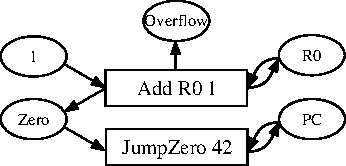
\includegraphics[width=2cm]{./img/ISA/addAndJump.pdf}
\caption{Data-flow graphs of instructions and short programs}
\label{fig-addAndJump-gcd}
\end{figure}

\subsubsection{\textbf{Simulation}}



\subsubsection{\textbf{Restrictions}}

